\documentclass[border=6pt]{standalone}
\usepackage{tikz}
\usetikzlibrary{arrows.meta,fit,backgrounds}
\usepackage{helvet}
\renewcommand{\familydefault}{\sfdefault}
\newcommand{\sys}{ActPlane}

\begin{document}
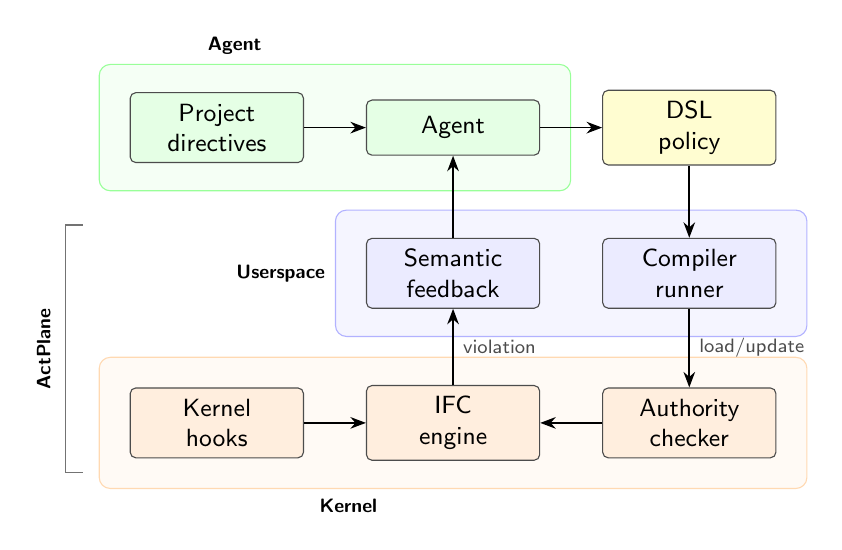
\begin{tikzpicture}[
  >=Stealth,
  box/.style={
    draw=black!70,
    rounded corners=2pt,
    minimum height=0.70cm,
    minimum width=2.20cm,
    align=center,
    font=\small,
    inner xsep=6pt,
    inner ysep=4pt
  },
  agent/.style={box, fill=green!10},
  user/.style={box, fill=blue!8},
  dsl/.style={box, fill=yellow!18},
  kernel/.style={box, fill=orange!13},
  arr/.style={->, line width=0.58pt},
  lbl/.style={font=\scriptsize, text=black!70},
]

% Agent layer.
\node[agent] (directive) at (-3.0,3.2) {Project\\directives};
\node[agent] (agent) at (0.0,3.2) {Agent};
\node[dsl] (policy) at (3.0,3.2) {DSL\\policy};

% Userspace.
\node[user] (feedback) at (0.0,1.35) {Semantic\\feedback};
\node[user] (compiler) at (3.0,1.35) {Compiler\\runner};

% Kernel.
\node[kernel] (hooks) at (-3.0,-0.55) {Kernel\\hooks};
\node[kernel] (engine) at (0.0,-0.55) {IFC\\engine};
\node[kernel] (authority) at (3.0,-0.55) {Authority\\checker};

% Policy update path.
\draw[arr] (directive) -- (agent);
\draw[arr] (agent) -- (policy);
\draw[arr] (policy) -- (compiler);
\draw[arr] (compiler) -- node[right,lbl] {load/update} (authority);
\draw[arr] (authority) -- (engine);

% Runtime enforcement path.
\draw[arr] (hooks) -- (engine);
\draw[arr] (engine) -- node[right,lbl] {violation} (feedback);
\draw[arr] (feedback) -- (agent);

\begin{scope}[on background layer]
  \node[fit=(directive)(agent), fill=green!4, draw=green!40,
        rounded corners=4pt, inner xsep=11pt, inner ysep=10pt,
        label={[font=\scriptsize\bfseries]above left:Agent}] {};
  \node[fit=(feedback)(compiler), fill=blue!4, draw=blue!30,
        rounded corners=4pt, inner xsep=11pt, inner ysep=10pt,
        label={[font=\scriptsize\bfseries]left:Userspace}] {};
  \node[fit=(hooks)(authority)(engine), fill=orange!4, draw=orange!30,
        rounded corners=4pt, inner xsep=11pt, inner ysep=10pt,
        label={[font=\scriptsize\bfseries]below left:Kernel}] {};
\end{scope}

\draw[draw=black!55, line width=0.6pt]
  (-4.70,1.96) -- (-4.92,1.96) -- (-4.92,-1.18) -- (-4.70,-1.18);
\node[font=\scriptsize\bfseries, rotate=90] at (-5.20,0.39) {\sys{}};

\end{tikzpicture}
\end{document}
